\documentclass[french, a4paper, 12pt]{article}

\newcommand{\docname}{Les disparus de Nurgundi}
\newcommand{\authorname}{Loris Delafosse et Antoine Royer}
\newcommand{\dmy}{}
\newcommand{\years}{2020 -- 2021}
\newcommand{\org}{Odyssée}

\input{~/latex/article.tex}

\usepackage{graphicx}
\begin{document} \maketitle \vspace{3pt} \hrule \vspace{3pt}

\tableofcontents



\section{Contexte}

Empire d'Otlin, frontière sud. Les troupes skorgaises se font de plus en plus oppressantes et la population otlinoise commence à vraiment souffrir des persécutions perpétrées par l'armée sur les villages.

Les soldats attaquent les populations civiles, réduisant les bourgs frontaliers à l'état de ruines fumantes, laissant en guise de champs de vastes cicatrices dans la terre brûlée et souillée du sang des villageois.

\section{Présentation du lieu}

\begin{figure}[htp]
\centering
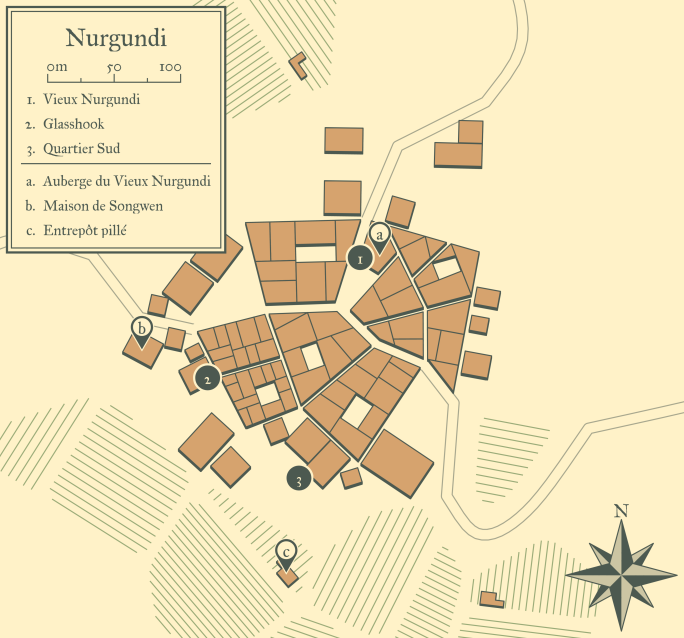
\includegraphics[scale=0.50]{nurgundi.png}
\caption{Nurgundi}
\end{figure}

Un des bourgs encore épargné est celui de Nurgundi. Situé à la limite des montagnes qui séparent les deux Empires.

Laissé sans citadelle ni mur, Nurgundi ne doit sa longévité qu'à sa position, assez enclavée. Mais les groupes de pillards skorgais se rapprochent, passant par les montagnes au sud et par les plaines à l'est. Pris en tenaille le bourg a demandé de l'aide au gouvernement otlinois, mais le temps presse et les troupes demandées sont encore à plus de 280 km et n'arriveront jamais à temps.

Les villageois construisent donc eux-mêmes leur défense, s'organisant en guets et patrouilles pour sécuriser le bourg et ses alentours.

\section{Intrigue}

Ces dernières semaines, l'activité débordante du bourg est vertigineuse. Tout le monde s'affaire à consolider les maisons, à faire des réserves d'eau ou de nourriture, à s'équiper. Tout ressemble à une arme, une pierre, un bout de bois, une vieille épée rouillée. Le peuple otlinois n'est pas prêt pour une guerre, surtout dans les campagnes.

Dans ce climat fébrile, personne ne s'est immédiatement rendu compte de la disparition du doyen du village, Songwen. On a alors pensé à une mort naturelle, ou alors il n'a pas voulu rester avec les combats imminents. Mais lorsque Laskim, sa femme, disparait à son tour, la tension monte. Au bout de plusieurs jours, le nombre de disparus augmente, et des évènements étranges se produisent : bruits, objets qui disparaissent ou changent de place… Diverses explications sont alors nées : pour certains il s'agit d'un coup des pillards skorkais pour terroriser Nurgundi, pour d'autre ce sont des signes des Dieux.

Au début, il ne s'agissait que d'une rumeur, mais aujourd'hui les villageois hésitent de plus en plus à quitter leur terre.

\section{Quête principale}

\subsection{Arrivée à Nurgundi}

Devant ces étranges évènements, la population effrayée à fait appel à Narcisse le Grand, éminent théologue otlinois, qui a consenti à se déplacer devant les supplications des habitants pour comprendre ces disparitions. Certaines légendes racontent que Narcisse le Grand est l'incarnation d'un Dieu du Panthéon de Rangorhe. Ce qui fait de lui une personnalité de premier plan quand il s'agit d'évènements surnaturels.

\subsection{Quête}

Vous devez calmer la population et donner une explication à tous ces évènements, avant l'attaque des pillards skorgais. Il vous reste donc un peu plus d'une semaine…


\end{document}